\documentclass[conference]{IEEEtran}
\usepackage[square,sort,comma,numbers]{natbib}
\bibliographystyle{unsrtnat}
\usepackage{amsmath,amssymb,amsfonts}
\usepackage{algorithmic}
\usepackage{graphicx}
\usepackage{textcomp}
\usepackage{xcolor}
\usepackage{fancyhdr}
\usepackage{array}
\usepackage{booktabs}
\usepackage{comment}
\newcommand\Tstrut{\rule{0pt}{2.6ex}}         % = `top' strut
\newcommand\Bstrut{\rule[-0.9ex]{0pt}{0pt}}   % = `bottom'
\pagestyle{fancy}
\fancyhf{}
\rhead{Analysis of Cognitive Load in Human Robot Interactions}
\lhead{University of the West of England }
\rfoot{Page \thepage}

\def\BibTeX{{\rm B\kern-.05em{\sc i\kern-.025em b}\kern-.08em
    T\kern-.1667em\lower.7ex\hbox{E}\kern-.125emX}}
\begin{document}

\title{Analysis of Cognitive Load in Human Robot Interactions}

\author{
	\IEEEauthorblockA{Simon Bluett, Alfie Sargent, Natalia Gonz\'alez Cadiente, Xuan Wang, Jinze Ding \\
	\textit{Human Robot Interaction - University of the West of England}}
}

\maketitle

\begin{abstract}
A user study was conducted to investigate cognitive load during human robot interaction with a Nao robot \cite{web:NaoRobot} \& video-based agent; the participants were given instructions to complete a task using an oscilloscope and waveform generator. Measurements taken during experimentation were: heart rate, GSR (Galvanic skin response), response time, task performance \& questionnaire results. \newline
The study itself was conducted at the Bristol Robotics Laboratory by 9 participants (age between 21-25, 5 men, 4 women) with mixed prior knowledge of the equipment used. Some participants interacted with the robot first, and some with the computer first. Participants were also tasked with a reaction task where they had to indicate when a screen began to fade to black. In between tasks, participants were given a questionnaire to answer as well as a questionnaire at the end. \newline
The results gathered show that there is a slight increase in GSR conductance when participants were given instructions by the robot, but it is not large enough to be considered a direct correlation. Overall, the difference in cognitive load when given from a robot or a computer is small, with most candidates completing the task faster when given by a computer. \newline
Results gathered do suggest a slight increase in cognitive load when interacting with a robot but more research needs to be done to comfortably conclude this. 
\end{abstract}
\section{Introduction}
Robotics is quickly becoming a part of every day life for many people with devices such as the Roomba \cite{web:roomba} \& Alfawise Magnetic \cite{web:alfawise} becoming increasingly popular. They offer the ability to autonomously complete tasks like cleaning the house; essentially increasing the standard of living for an individual. They also have other benefits such as helping disabled individuals through assistive robotics\cite{mataric2007socially} and educating children with autism \cite{shamsuddin2012initial}. All of these examples require the human to interact with the robot; human robot interaction. \newline
As robotics becomes more quotidian, the way people interact with these robots should be investigated to ensure the best design is implemented. Cognitive load refers to the used amount of working memory resources when completing a task. For more robotic devices to be welcomed into the general populace, the cognitive load during human robot interactions should be researched. \newline

In this study we aim to investigate the cognitive load of a user during human robot interaction with a Nao robot in comparison to a video-based agent. This will be done by having participants complete a task with instructions given by a physical Nao robot and a computer, monitoring physiological data during the task as well as a questionnaire at the end to determine cognitive load. 

\section{Related Work}
\subsection{Cognitive Load Theory}
Based on prevailing cognitive load theory \cite{deleeuw2008comparison,de2010cognitive,sweller1994cognitive}, there are 3 types of cognitive processing when learning: extraneous processing, intrinsic processing and germane processing (see Table~\ref{Tabel:1}). Each type of cognitive load will be measured in this user study. 
\begin{table*}[h!]
    \caption{A table detailing the 3 types of cognitive load \cite{deleeuw2008comparison,de2010cognitive}.}
    \label{Tabel:1}
    \centering
    \begin{tabular}{| p{8em} | p{8cm}| p{6cm} |}
     \hline\Tstrut
     \textbf{Cognition type} & \textbf{Description} & \textbf{Example} \\ [0.5ex] 
      \hline\hline\Tstrut
       \textit{Extraneous} & Predominately caused by inappropriate or frustrating instructional design that ignores the natural working limits of human memory. & An educational book that isn't well laid out, requiring the read to go back and forth. \\
         \hline\Tstrut
        \textit{Intrinsic} & Caused by the natural structure and complexity of the topic being covered; the inherent load required to learn something. & The calculation of  $2+2=4$ has a lower load than more advanced mathematics like calculus.\\
         \hline\Tstrut
       \textit{Germane} & A deeper cognitive learning process that involves the individual mentally organising what has been learned for cognitive access later; this is often described as being organised into a schema \cite{paas2003cognitive}.& Understanding the relationship between topics like how the algorithms used in one programming language can be used in another; forming a connection in long term memory and strengthen that connection.\\
         \hline
    \end{tabular}
\end{table*}

\subsection{Cognitive Load Measurements}
\citet{deleeuw2008comparison} investigated the cognitive load of 155 college students with limited engineering knowledge when attending a lesson on electric motors. The lesson also involved a secondary distraction task, which monitored the awareness of participants. The cognitive load was measured by: a preliminary questionnaire, response time to the secondary task, 8 self-report scales throughout experimentation and a final questionnaire. The results created are consistent with the prevailing theory \cite{ayres2006using}; that different features of cognitive load can only be accessed by different measurement techniques. For example, extraneous load was identified using the response time of subjects, while germane load was measured using difficulty-rating questionnaires. 

The measuring techniques in our study emulated many of the methods used by \citet{deleeuw2008comparison}, but did not require participants to report their own cognition during the study to avoid tampering with other measurements. Furthermore, biometric measurements were employed to provide additional, non-subjective indicators of cognitive load.

Several papers have examined the physiological effects that cognitive load can have on individuals such as eye position tracking \cite{palinko2010estimating}, relative blood flow \cite{ikehara2005assessing} and pupil size \cite{partala2003pupil}. The most prominent measurement which suggests a proportionality with cognitive load is galvanic skin response (GSR)---a measure of skin conductance \cite{shi2007galvanic,nourbakhsh2012using}. 

\citet{ikehara2005assessing} performed a study using GSR, consisting of 13 male US air force volunteers aged between 18-21. The participants were shown a set of fractions moving across a computer screen, and were tasked with selecting fractions greater than a 1/3 before they hit the right side of the screen (Figure~\ref{fig:MovingfracitonsTask}). The participant would gain points for choosing correctly, and lose points for not selecting in time or selecting the wrong fraction.

\begin{figure}[h!]
    \centering
    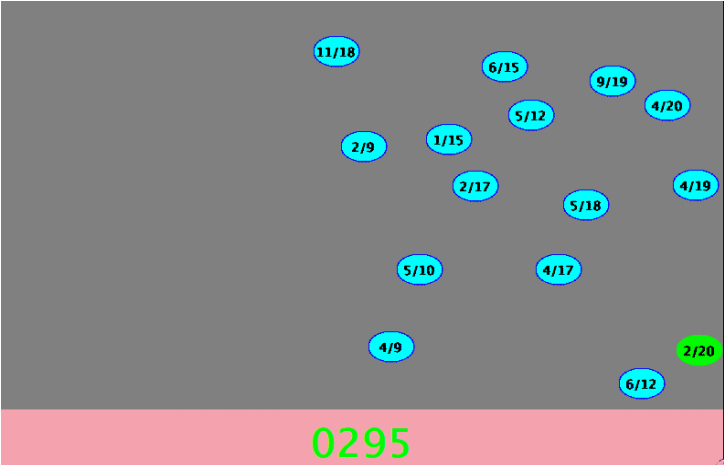
\includegraphics[width=0.95\linewidth]{figures/ScreenCaptureFractions.PNG}
    \caption{Screen capture of the moving fractions task \cite{ikehara2005assessing}.}
    \label{fig:MovingfracitonsTask}
\end{figure}

The GSR results showed that the device was capable of detecting a decrease in sweat cell arousal as the complexity of the task increased. The study used a bespoke physiological measuring device with little detail on its development. It was applied to the participants left hand, with no indication of which hand was preferred by the user, potentially changing the results especially considering the experiment required participants to actively use their hand. In our study, a professional GSR sensor was placed on the non-dominant hand, and the participant's hand was be kept stationary throughout the experiment.

\subsection{HRI vs Video Displayed Agents}
\citet{bainbridge2011benefits} investigated how a robot's physical presence can affect a human's judgement when handling physical objects. In the experiment, 65 university staff, graduates and undergraduates were tasked with relocating books in a room; 22 had the robot physically with them (as shown in Figure \ref{fig:nico_experimentl}), 22 had a live feed of the robot and 21 had an augmented video of the robot. The results show the participants had a greater ``respect'' for the robot's sense of space and would actively go out of their way to avoid the robot's space.

Furthermore, the study showed an increase in ``trust'' if the task was given by a physical robot. Although this experiment was focused solely on social interaction and not cognitive load, the results gathered are still relevant to the user study being created. The mention of personal space and trust being greater with the presence of a robot may be indicative of cognitive load as well; this will be studied further in the experiment being designed.

\begin{figure}[h!]
    \centering
    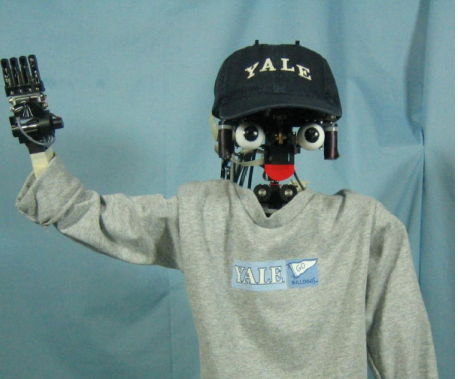
\includegraphics[width=0.95\linewidth]{figures/Nico.PNG}
    \caption{\label{fig:nico_experimentl}Nico, the robot used by \citet{bainbridge2011benefits}. Participants were more willing to follow orders given by Nico.}
\end{figure} 

\section{Methods}

\subsection{Hypotheses}
The main research question of the study is: Does the introduction of a physically embodied robot increase cognitive load when interacting with humans to complete a complex task? Our hypothesis is that introducing a robot into the learning process of a complex task will increase cognitive load and therefore hinder the ability to complete the task.

The way in which we measure the hypothesis is to firstly ask participants to fill out questionnaires indicating their stresses, preferences and overall thoughts on their experience. Secondly, we conduct physiological tests looking at skin conductance, heart rate and reaction times to an awareness test; slow reaction times and increased heart rate will indicate increased cognitive load of the participant. 

\subsection{Validity and  Reliability}

\subsubsection{Internal validity} 
Internal validity is controlled by randomising the order of the tasks and ensuring participants have not seen the study prior to taking part. This means participants aren't affected due to learning how the robot behaves and preparing for the study. Selection effects are avoided by randomly selecting participants so that not all participants have the same knowledge and background. For this study, it was found that many of the users had previous experience with some form of robot in their life and therefore this may affect the internal validity. To remove experimental bias in which those conducting the study influence the outcome, the same guidelines are provided for both robot and computer scenarios, and the computer uses the same voice as the robot when giving instructions. The guidelines are given on paper to avoid indicating preference to the participant.

\subsubsection{External validity}
Environmental influences include other studies being run in the same room, many people watching, and outside noise that may cause disturbance to the participant. In real-life scenarios, outside noise and other humans nearby may increase the generalisability of this study. External validity could be further increased by testing different sub-groups, for example including participants of a wider age range and background.

\subsubsection{Reliability}
9 participants were studied in this research. Participants had a variety of backgrounds and experiences with both the oscilloscope equipment and robot interaction. Studying more participants would increase the reliability and repeatability of the study, providing more conclusive results. Uncontrolled variations also affected the reliability of the study. Most users had some experience with robots or the oscilloscope equipment. More reliable results would include users with varying prior experience.

\subsection{User Study Design}
The study was designed to take into consideration the three categories of cognitive load. The task consisted of operating a oscilloscope and waveform generator, whose complex array of buttons and dials should provide an intrinsic cognitive load to people who are not familiar with the equipment. 

The extraneous cognitive load comes from the demands by the teacher or instructions; how the information is presented. This type of cognitive load inhibits the humans ability to learn and successfully complete tasks and is therefore the type of load a robot may influence. We deliver some instructions via a robot, and others via a computer to analyse the changes in cognitive load in human-robot interaction.

A within user study design is chosen due to the limited number of users available to participate within the time frame. This is to allow us to gather sufficient results for analysis. The study works by alternating which test condition the user is exposed to first; robot or computer.

\subsection{User Study Procedure}
The participant is guided through the task of creating a waveform using the equipment provided in 8 steps. Four steps are presented by the robot, and four by the computer. Throughout this, the participant must complete an awareness task.

\subsubsection{Awareness Task}
We set a cognitive load baseline by using an awareness task. The users are asked to pay attention to a computer whose screen changes colour periodically. When the screen changes to black, the participant must press the spacebar. The users heart rate and skin conductance are measured, and the number of correct and incorrect key presses by the user are recorded.
This task is used before the test to create a baseline, and during both computer and robot stages of the study.

\subsubsection{Questionnaires}
Three questionnaires are used throughout the study:
\begin{itemize}
    \item Pre-study Questionnaire: Questions regarding age, demographic, equipment experience, and robot experience
    \item Mid- and Post-study Questionnaire: The same questionnaire presented separately, after the robot condition and after the computer condition. Questions regarding frustration levels, understanding of the task, how well they have learned the task. (NASA TLX style)
    \item Mid- and Post-study Interview: Pre-written questions regarding opinions of the robot/computer, suggested improvements, and thoughts on the task itself.
\end{itemize}

\subsection{Dependent Measures}
\begin{itemize}
    \item NASA TLX style questionnaire \cite{hart1988development}
    \item Galvanic Skin Response (GSR) and Heart Rate
    \item Awareness Test
    \item Time taken to complete the tasks
    \item Number of times the instructions had to be repeated
    \item The successful completion of each of the tasks
\end{itemize}
\subsection{Independent Variables}
\begin{itemize}
    \item Robot or Computer first
\end{itemize}

\section{Datasets and Results}

\subsection{Participants}

The experiment was conducted at the Bristol Robotics Laboratory and it was attended by randomly selected 5 men and 4 women. Participants were aged between 21-25, and 66.7\% (N=5) of them were native English speakers. The pre-survey questionnaire showed that 3 of them had no relevant human-robot interaction experience, and had not heard of the robot `NAO'. Only one participant indicated that they would not be interested in having a service robot in their home. Since the participants’ academic background and training could also influence their cognitive load during the study, the participants were asked about their familiarity with the devices (oscilloscope and waveform generator) being used throughout the study; more than half were unfamiliar with the the devices being used. The duration of each trial was approximately 15 minutes. During the experiment, the biometric data of the participants, such as heart rate, skin conductance, and skin resistance was recorded using a \textit{Shimmer} sensor. In subsequent sections, this data and the results from the questionnaires are recorded, and overall trends analysed. 
\subsection{Physiological Data}
Skin conductive, skin resistance \& heart rate were recorded for 9 participants during both robot and computer experiments. Baseline data was recorded for 30 seconds before each of the experiments. The change of those parameters are presented. \newline
\subsubsection{Galvanic skin conductance} The result showed that the skin conductance difference of the robot instructions ($\mu$ = 2.23, $\sigma$ = 3.09) were higher than that of the computer instructions ($\mu$ = 1.59, $\sigma$ = 1.43). The average skin conductance of 6 of the participants during the robot instruction was higher than the computer instruction. Figure \ref{fig:skin_conductance} illustrates the skin conductance of each of the participants.

\begin{figure}[h]
	\flushleft 
	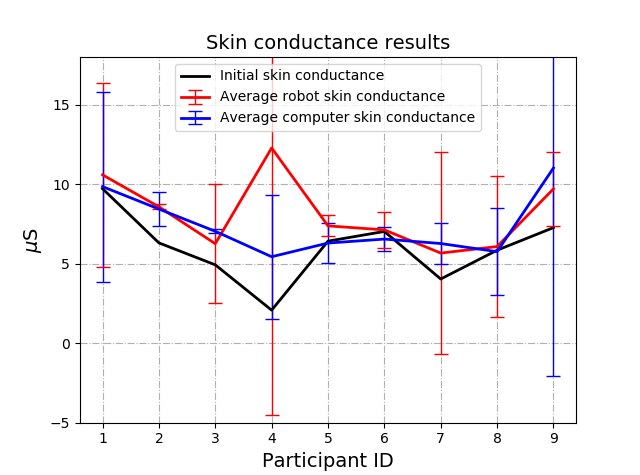
\includegraphics[width=1\linewidth]{figures/conductance.png}
	\caption{\label{fig:skin_conductance}Galvanic skin conductance values for all participants.}  
\end{figure}


\subsubsection{Heart rate} The average heart rate of subjects during robot instructions ($\mu$ = 88.64BPM, $\sigma$ = 1.596) was on par with those during the computer instructions ($\mu$ = 88.62BPM, $\sigma$ = 2.495). The average heart rate is shown in Figure \ref{fig:heart_rate}.

\begin{figure}[h]
	\flushleft 
	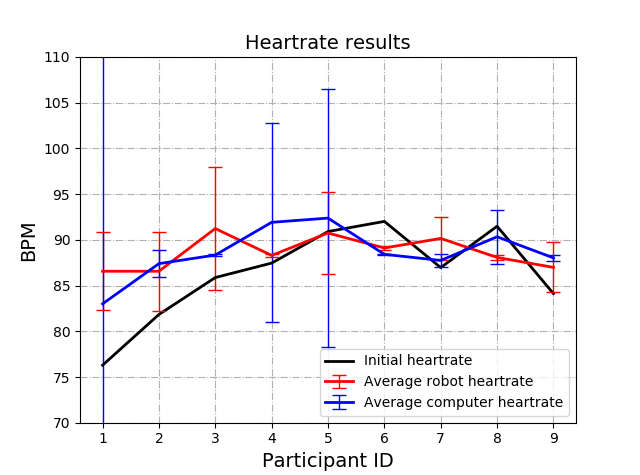
\includegraphics[width=1\linewidth]{figures/heartrate.png}
	\caption{\label{fig:heart_rate}Heart rate values for all participants.}  
\end{figure}

\subsection{Awareness Task}
Figure \ref{fig:awareness_reaction} illustrates the average reaction times of each participant to pressing the keyboard when the awareness test screen turned black. The results for the first four subjects was not recorded properly, so they have been excluded. The reaction time tended to be slower during the robot scenario, relative to the computer (Avg. increase of +488.5ms, $\sigma$ = 837.7). The subjects detected a lower percentage of the black screens during the robot instructions ($\mu$ = 0.38, $\sigma$  = 0.387) compared to the computer ($\mu$ = 0.5, $\sigma$  = 0.400).

\begin{figure}[h]
	\flushleft 
	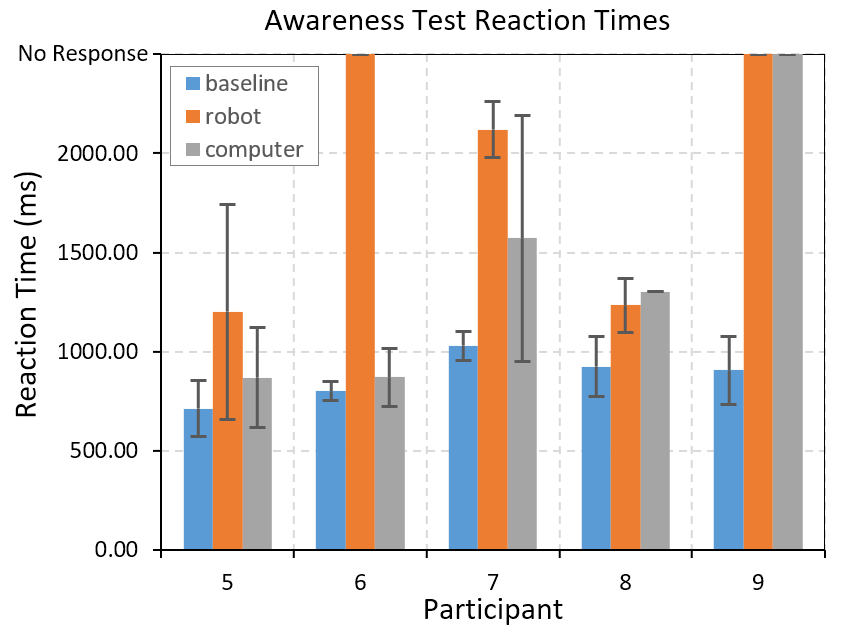
\includegraphics[width=1\linewidth]{figures/awareness_reactions.png}
	\caption{\label{fig:awareness_reaction}Reaction time of participants responding to the awareness task.}  
\end{figure}

\subsection{Instruction Completion Times}

Figure \ref{fig:instruction_time_diff} shows the average time differences of completing the computer instructions, relative to the robot instructions. In general, the computer instructions were completed more quickly ($\mu$ = -2912ms, $\sigma$ = 6328). It was also found that the second set of instructions tended to take more time to complete, relative to the first set ($\mu$ = +5202ms, $\sigma$ = 4125).
\begin{figure}[h]
	\flushleft 
	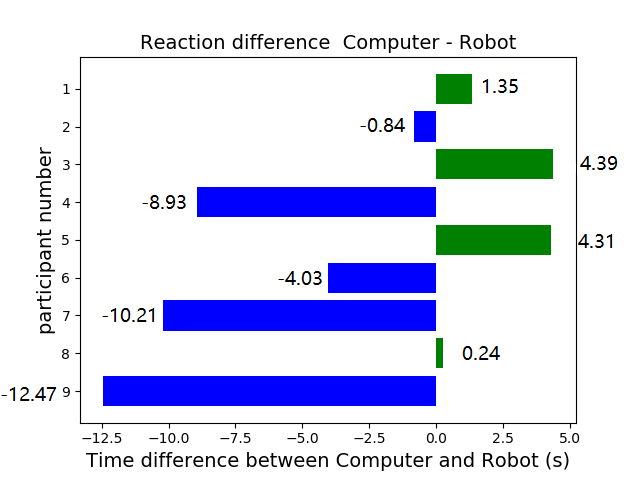
\includegraphics[width=0.95\linewidth]{figures/difference.png}
	\caption{\label{fig:instruction_time_diff}Average time difference for each participants to complete the tasks.}  
\end{figure}

\subsection{Post experiment questionnaire}
For each robot and computer experiment, the participants answered 7 question by the degree from 1 to 5. The average point value of the questions are presented Table \ref{tab:questionairre}.   

\begin{table}[h]
\caption{\label{tab:questionairre}Average scores}
\begin{tabular}{|c|c|c|c|}
\hline
\multicolumn{1}{l|}{No} & \multicolumn{1}{l|}{}                                                                                                          & \multicolumn{1}{l|}{Robot} & \multicolumn{1}{l|}{Computer} \\
\hline \hline
1                       & \begin{tabular}[c]{@{}c@{}}How would you rate your experience with \\ the equipment used? \end{tabular} & 3.875                      & 4.375                         \\ \hline
2                       & \begin{tabular}[c]{@{}c@{}}How difficult did you find the tasks?\end{tabular}                                               & 2.625                      & 1.75                          \\ \hline
3                       & Were the instructions given clear?                                                                                             & 3.5                        & 3.875                         \\ \hline
4                       & \begin{tabular}[c]{@{}c@{}}How frustrated did you feel during \\ the tasks?\end{tabular}                                       & 2.375                      & 1.75                          \\ \hline
5                       & \begin{tabular}[c]{@{}c@{}}How competently do you think you\\  completed the tasks assigned?\end{tabular}                      & 3.5                        & 4.125                         \\ \hline
6                       & \begin{tabular}[c]{@{}c@{}}How much more guidance would you need \\ if you were to do the task again?\end{tabular}             & 2.75                       & 1.875                         \\ \hline
7                       & \begin{tabular}[c]{@{}c@{}}How confident are you now in\\  completing the task unassisted?\end{tabular}                       & 3.5                        & 4                             \\ \hline

\end{tabular}
\end{table}

The distribution of scores for each participant is presented in Figure \ref{fig:questionnaire_distrib_1} and Figure \ref{fig:questionnaire_distrib_2}; one person's results is not showed because he/she didn't complete the task successfully and most questions were rated as unknown.

\begin{figure}[h]
	\flushleft 
	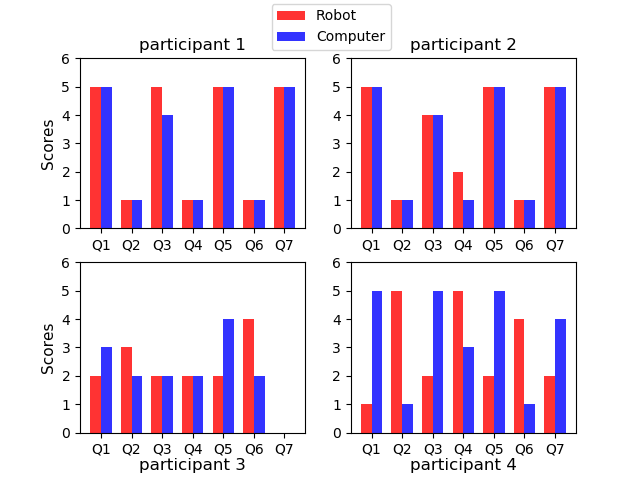
\includegraphics[width=1.05\linewidth]{figures/first.png}
	\caption{\label{fig:questionnaire_distrib_1}Questionnaire result for first group of participants.}
\end{figure}

\begin{figure}[h]
	\flushleft 
	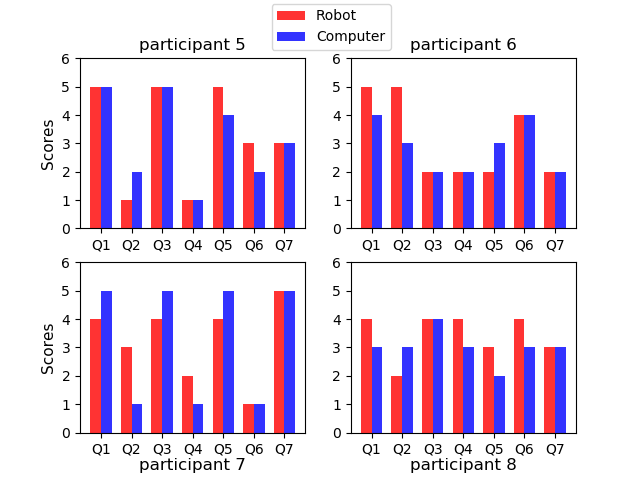
\includegraphics[width=1.05\linewidth]{figures/last.png}
	\caption{\label{fig:questionnaire_distrib_2}Questionnaire result for second group of participants.}
\end{figure}

\subsection{Post Experiment Interview}
Five participants claimed no significant difference between the instructions provided by the robot and the computer, but due to the complexity of the mission, they indicated that they did not pay much attention to the robot. In contrast, the questionnaire showed that the computer instructions required less attention. Only one person preferred the robot interaction to the computer one. Two participants stated that their understanding of the instructions was aided by the NAO’s gestures, while two other participants stated that the robot's instructions were hard to follow. 

\section{Discussion}
\begin{comment}
THIS FIRST PARAGRAPH SHOULD BE ABOUT BIG PICTURE STUFF, WHY THE STUDY IS IMPORTANT\newline
Summarize the major gap in understanding that your work is attempting to fill. What was the overarching hypothesis?\newline
Why is filling this gap important? How will answering this question move the field forward? \newline
\end{comment}
 The hypothesis of this study was "Does the introduction of a physically embodied robot increase cognitive load when interacting with humans to complete a complex task?". The way that humans interact with robots is essential to designing competent robotic systems \& a key aspect of that is exploring a humans cognitive load during interaction, which has been done in this study. By understanding the underlying cognitive effects that human robot interaction has on a person, systems can be modelled to suit the cognitive needs of the task \& consequently be more effective in operation. This becomes more prevalent dependent on the task such as education, you need to ensure that the student remains engaged with what is being taught and thus you want the intrinsic and germane cognitive load to be high \& the extraneous cognitive load to be low.\newline
 
\begin{comment}
THE SECOND PARAGRAPH SHOULD BE ABOUT THE CRITICAL ANALYSIS OF THE MAJOR FINDINGS OF THE RESULTS\newline
What was your overall approach for studying the gap? \newline
What was the most important result of your study?\newline
How does your result(s) fit with existing literature?\newline
\end{comment}
The physiological data that was gathered was mostly inconclusive, with the heart rate being almost identical for the interaction with the Nao robot and the computer. Although there was a slight increase in skin conductivity when participants interacted with the robot, it is not significant enough to be considered a direct correlation with cognitive load. Moreover, he results gathered are not entirely reliable considering participant 4 had such drastically different conductance values. Overall, the bio-metric data suggests a slight increase in skin conductivity which is indicative of an increased cognitive load but it is not conclusive enough to matter state, with certainty, that the robot produced a higher cognitive load.\newline

The reaction time measured during the "distraction" task did produce some interesting results. For each participant, the reaction time was slower when the robot was being used, suggesting an increased extraneous cognitive load. It is worth noting that participants 6,7 and 9 had not used a Nao robot before and there reaction time was significantly lower in its presence, by a factor of 3 in some cases. This data is also reflected in the questionnaires, where 8 of the 9 participants preferred he computer based task. This indicates that the cognitive load was higher when the robot was used but not for productive cognition, the participants preferred the computer because it was less distracting. Unfortunately, 4 participants data was corrupted and as a result, any observations drawn from the reaction task are not reliable; further research is needed. \newline

Lastly, the mean values for the questionnaire state that people found the tasks more difficult when using the robot by almost 1 whole point. The overall conclusions drawn from the questionnaire results are that the participants found the instructions clearer and less frustrating when given by a computer. Furthermore, participants felt more competent in the task if the instructions were given by a computer suggesting a possible negative social aspect to the robot interaction.\newline

Although the study did produce some interesting results the overall conclusion is that the findings were inconclusive and further study must be done to determine the cognitive load during human robot interaction. Furthermore, the results may have had influencers on external validity which may have made the results less reliable. For example, the environment in which the study was held was not conducive for a good experiment; distractions from other people in the room and other noises may have affected the users ability to concentrate on the task and therefore changed the results. Future studies in this field must make the environmental conditions less distracting so that the task can be completed properly.\newline Moreover, although precautions were taken to increase the reliability of the bio-metric data gathered such as making sure the user kept there hand still during operation, the sensor that was used produced many errors that resulted in some of the data becoming corrupted and inaccessible for review. Future researchers should ensure that the device they are using has been properly tested and researched prior to the experiment. \newline

Overall, the results are inconclusive due to the small number of participants and the loss of data throughout the experiment but the data that has been gathered suggests a slight increase in cognitive load when using a robot over a video displayed agent but it is not conclusive. Current studies \cite{bainbridge2011benefits} suggest that human robot interaction results in a large cognitive load but due to experimental errors and lack of significant, valid and reliable results, the experiment cannot support or oppose this.


% _________________________________________________________________________________
%% Conclusion (PERSONAL)
% ^^^^^^^^^^^^^^^^^^^^^^^^^^^^^^^^^^^^^^^^^^^^^^^^^^^^^^^^^^^^^^^^^^^^^^^^^^^^^^^^^
\section{Conclusion}
The results gathered and analyzed suggest a slight increase in cognitive load when a robot gives instructions to a human but it is not conclusive and further research needs to be done to confirm this. However, this does create a precedent for future research in this field.\newline
Future research in this field should explore how a more engaging and intimate robot effect people levels of cognition. Ultimately the robot that was used in this experiment was not interactive enough with the participant themselves, the system should be more complex with more social queues such as complex movement, gestures, Furthermore, future work could research how a robotic system effects people who have less familiarity with robotics; many of the participants in this experiment already had some level of familiarity with the robot and the equipment that was being used. Lastly, the method in which cognitive load was measured could be considered intrusive and consequently effected the results gathered. Future work could look into measuring cognitive load in a non intrusive way. \newline

Overall, the study itself did produce some interesting results but is in no way conclusive for this field, further work needs to be done to determine how human robot interaction effects the cognitive load of the user. This is a worthy research topic because it ultimately leads to more efficient robotic systems being developed.
% _________________________________________________________________________________
\bibliography{refs}
\end{document}

